\documentclass[]{article}
\usepackage{lmodern}
\usepackage{amssymb,amsmath}
\usepackage{ifxetex,ifluatex}
\usepackage{fixltx2e} % provides \textsubscript
\ifnum 0\ifxetex 1\fi\ifluatex 1\fi=0 % if pdftex
  \usepackage[T1]{fontenc}
  \usepackage[utf8]{inputenc}
\else % if luatex or xelatex
  \ifxetex
    \usepackage{mathspec}
  \else
    \usepackage{fontspec}
  \fi
  \defaultfontfeatures{Ligatures=TeX,Scale=MatchLowercase}
\fi
% use upquote if available, for straight quotes in verbatim environments
\IfFileExists{upquote.sty}{\usepackage{upquote}}{}
% use microtype if available
\IfFileExists{microtype.sty}{%
\usepackage{microtype}
\UseMicrotypeSet[protrusion]{basicmath} % disable protrusion for tt fonts
}{}
\usepackage[margin=1in]{geometry}
\usepackage{hyperref}
\hypersetup{unicode=true,
            pdftitle={Erik's Covid-19 Chart Pack},
            pdfborder={0 0 0},
            breaklinks=true}
\urlstyle{same}  % don't use monospace font for urls
\usepackage{graphicx,grffile}
\makeatletter
\def\maxwidth{\ifdim\Gin@nat@width>\linewidth\linewidth\else\Gin@nat@width\fi}
\def\maxheight{\ifdim\Gin@nat@height>\textheight\textheight\else\Gin@nat@height\fi}
\makeatother
% Scale images if necessary, so that they will not overflow the page
% margins by default, and it is still possible to overwrite the defaults
% using explicit options in \includegraphics[width, height, ...]{}
\setkeys{Gin}{width=\maxwidth,height=\maxheight,keepaspectratio}
\IfFileExists{parskip.sty}{%
\usepackage{parskip}
}{% else
\setlength{\parindent}{0pt}
\setlength{\parskip}{6pt plus 2pt minus 1pt}
}
\setlength{\emergencystretch}{3em}  % prevent overfull lines
\providecommand{\tightlist}{%
  \setlength{\itemsep}{0pt}\setlength{\parskip}{0pt}}
\setcounter{secnumdepth}{0}
% Redefines (sub)paragraphs to behave more like sections
\ifx\paragraph\undefined\else
\let\oldparagraph\paragraph
\renewcommand{\paragraph}[1]{\oldparagraph{#1}\mbox{}}
\fi
\ifx\subparagraph\undefined\else
\let\oldsubparagraph\subparagraph
\renewcommand{\subparagraph}[1]{\oldsubparagraph{#1}\mbox{}}
\fi

%%% Use protect on footnotes to avoid problems with footnotes in titles
\let\rmarkdownfootnote\footnote%
\def\footnote{\protect\rmarkdownfootnote}

%%% Change title format to be more compact
\usepackage{titling}

% Create subtitle command for use in maketitle
\providecommand{\subtitle}[1]{
  \posttitle{
    \begin{center}\large#1\end{center}
    }
}

\setlength{\droptitle}{-2em}

  \title{Erik's Covid-19 Chart Pack}
    \pretitle{\vspace{\droptitle}\centering\huge}
  \posttitle{\par}
    \author{}
    \preauthor{}\postauthor{}
    \date{}
    \predate{}\postdate{}
  
\usepackage{booktabs}
\usepackage{longtable}
\usepackage{array}
\usepackage{multirow}
\usepackage{wrapfig}
\usepackage{float}
\usepackage{colortbl}
\usepackage{pdflscape}
\usepackage{tabu}
\usepackage{threeparttable}
\usepackage{threeparttablex}
\usepackage[normalem]{ulem}
\usepackage{makecell}
\usepackage{xcolor}

\begin{document}
\maketitle

Data updated 2020-06-20 19:00:33. World data are from
\href{https://github.com/NovelCovid/API}{Worldometers}. National and
state-level mortality, case, and testing data are from
\href{https://covidtracking.com}{Johns-Hopkins University}. County and
city-level mortality and case data are from the
\href{https://github.com/NovelCovid/API}{New York Times}. Most data
presented in this report were accessed through APIs provided by
\href{https://covidtracking.com}{The COVID Tracking Project} and
\href{https://github.com/NovelCovid/API}{NovelCOVID API}.

\hypertarget{world-data}{%
\section{World Data}\label{world-data}}

There have been 8,750,990 confirmed Covid-19 cases and 461,820 deaths
worldwide.

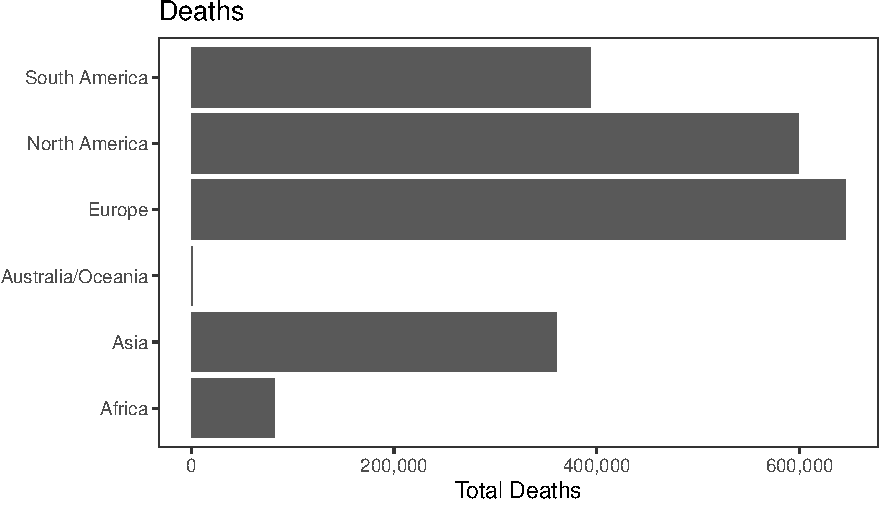
\includegraphics{covid_files/figure-latex/unnamed-chunk-1-1.pdf}

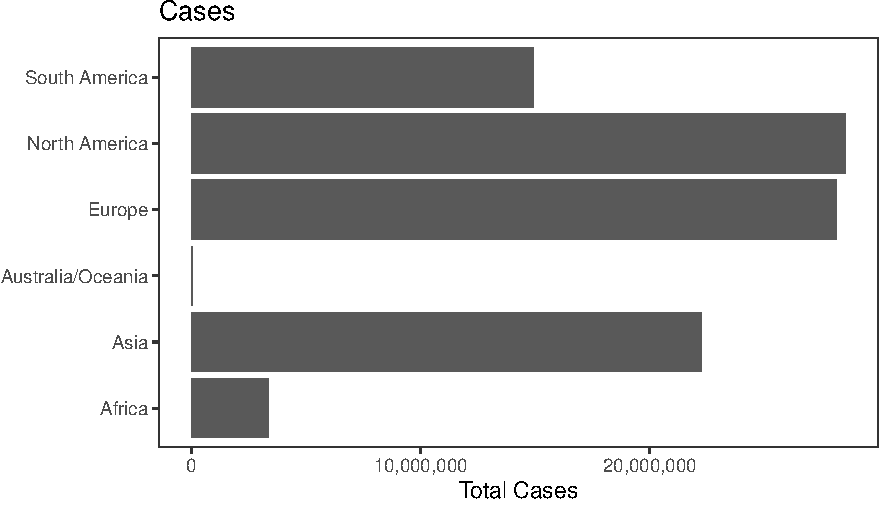
\includegraphics{covid_files/figure-latex/unnamed-chunk-2-1.pdf}

\newpage

\includegraphics{covid_files/figure-latex/unnamed-chunk-3-1.pdf}

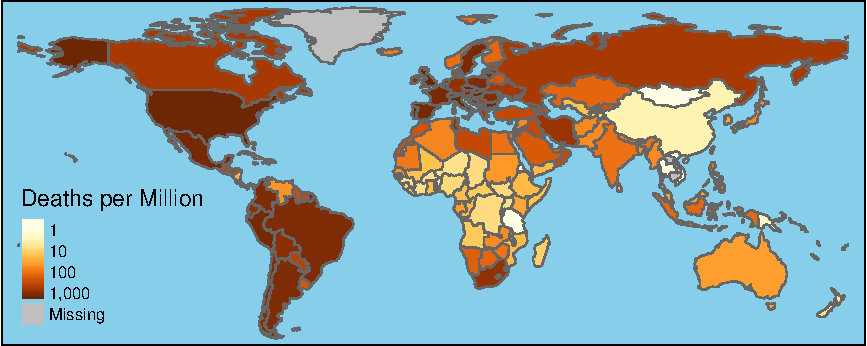
\includegraphics{covid_files/figure-latex/unnamed-chunk-4-1.pdf}

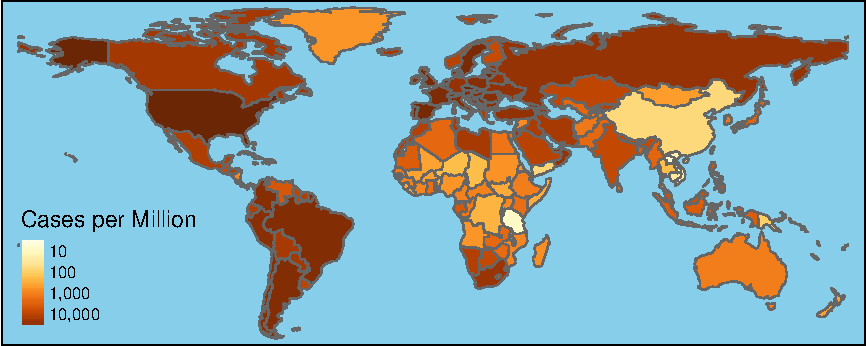
\includegraphics{covid_files/figure-latex/unnamed-chunk-5-1.pdf}

\newpage

\hypertarget{national-data}{%
\section{National Data}\label{national-data}}

There have been 2,241,990 confirmed Covid-19 cases and 113,452 deaths in
the United States.

\hypertarget{deaths}{%
\subsection{Deaths}\label{deaths}}

Because the effects of the virus can take several weeks to manifest in
patients, deaths are a lagging indicator of contagion, but they may be a
more reliable than case counts, which are a function of both the
prevalence of the disease and the rate of testing.

\includegraphics{covid_files/figure-latex/unnamed-chunk-7-1.pdf}

\includegraphics{covid_files/figure-latex/unnamed-chunk-8-1.pdf}

The case mortality rate is a very crude indicator of lethality because a
large numbers of non-lethal cases are likely never detected. A declining
case mortality rate is indicative of more widespread testing.

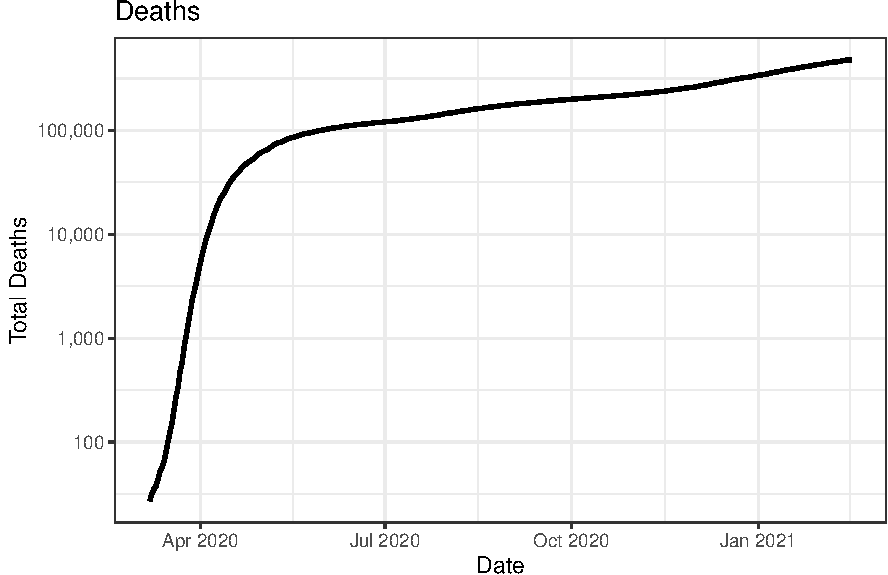
\includegraphics{covid_files/figure-latex/unnamed-chunk-9-1.pdf}

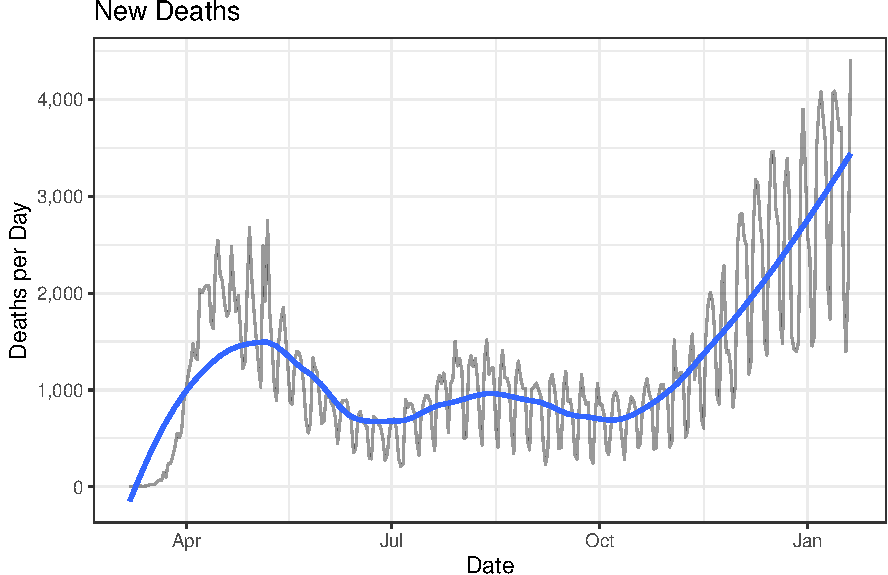
\includegraphics{covid_files/figure-latex/unnamed-chunk-10-1.pdf}

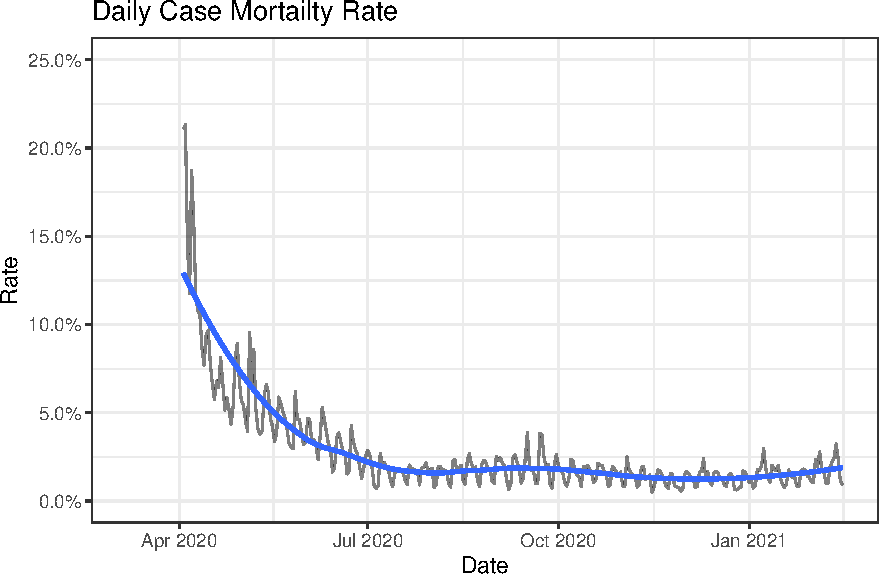
\includegraphics{covid_files/figure-latex/unnamed-chunk-11-1.pdf}

\newpage

\hypertarget{cases}{%
\subsection{Cases}\label{cases}}

Reported cases are a function of both the spread of the disease and the
prevalence of testing.

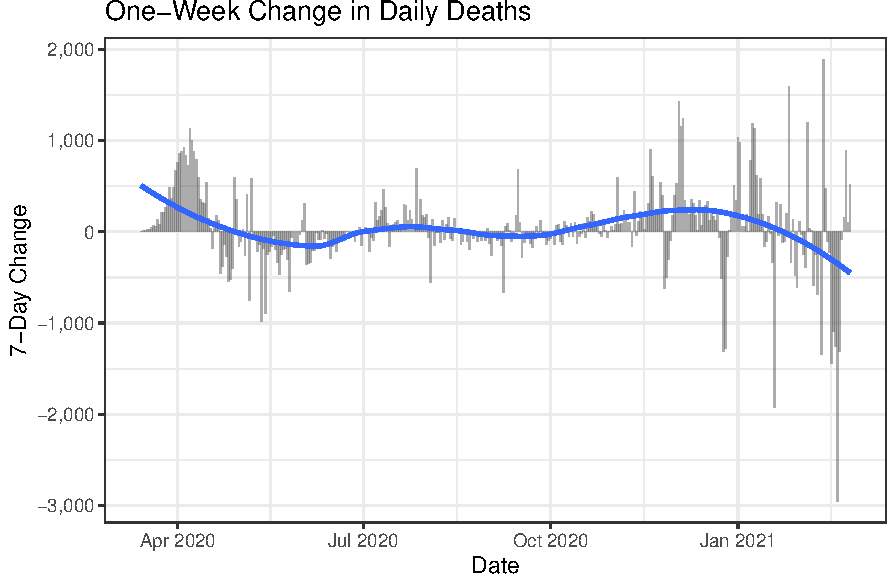
\includegraphics{covid_files/figure-latex/unnamed-chunk-12-1.pdf}

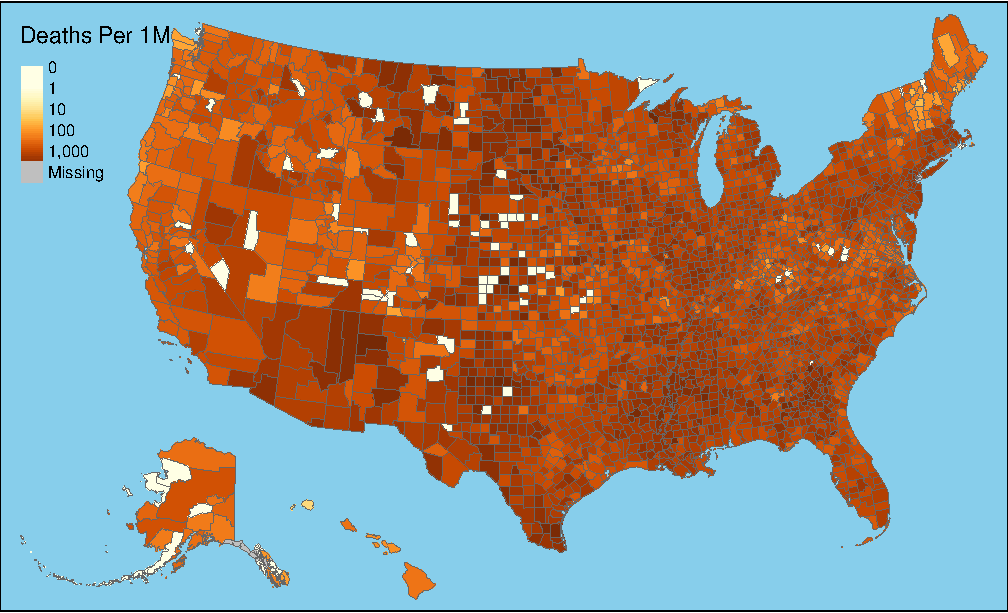
\includegraphics{covid_files/figure-latex/unnamed-chunk-13-1.pdf}

\includegraphics{covid_files/figure-latex/unnamed-chunk-14-1.pdf}

\includegraphics{covid_files/figure-latex/unnamed-chunk-15-1.pdf}

\newpage

\hypertarget{testing}{%
\subsection{Testing}\label{testing}}

Widespread testing is necessary for managing the spread of the disease.
The following charts show how testing in the United States has changed
over time.

\includegraphics{covid_files/figure-latex/unnamed-chunk-16-1.pdf}

\includegraphics{covid_files/figure-latex/unnamed-chunk-17-1.pdf}

When the supply of available tests is limited, they are typically only
used for patients whose symptoms suggest they are likely to have
contracted the virus. A high positive test rate indicates that testing
capacity is constrained.

\includegraphics{covid_files/figure-latex/unnamed-chunk-18-1.pdf}

\includegraphics{covid_files/figure-latex/unnamed-chunk-19-1.pdf}

\newpage

\hypertarget{state-data}{%
\section{State Data}\label{state-data}}

This section summarizes state-level data. Most data are reported for the
largest 15 states by population, which account for NaN percent of the
total U.S. population.

\hypertarget{deaths-1}{%
\subsection{Deaths}\label{deaths-1}}

\includegraphics{covid_files/figure-latex/unnamed-chunk-22-1.pdf}

\includegraphics{covid_files/figure-latex/unnamed-chunk-23-1.pdf}

\includegraphics{covid_files/figure-latex/unnamed-chunk-24-1.pdf}
\newpage

\includegraphics{covid_files/figure-latex/unnamed-chunk-25-1.pdf}

\includegraphics{covid_files/figure-latex/unnamed-chunk-26-1.pdf}

\newpage

\hypertarget{cases-1}{%
\subsection{Cases}\label{cases-1}}

\includegraphics{covid_files/figure-latex/unnamed-chunk-28-1.pdf}

\includegraphics{covid_files/figure-latex/unnamed-chunk-29-1.pdf}

\includegraphics{covid_files/figure-latex/unnamed-chunk-30-1.pdf}
\newpage

\includegraphics{covid_files/figure-latex/unnamed-chunk-31-1.pdf}

\includegraphics{covid_files/figure-latex/unnamed-chunk-32-1.pdf}

\newpage

\hypertarget{testing-1}{%
\subsection{Testing}\label{testing-1}}

\includegraphics{covid_files/figure-latex/unnamed-chunk-33-1.pdf}

\includegraphics{covid_files/figure-latex/unnamed-chunk-34-1.pdf}

\newpage

\includegraphics{covid_files/figure-latex/unnamed-chunk-35-1.pdf}

\includegraphics{covid_files/figure-latex/unnamed-chunk-36-1.pdf}
\newpage

Interpretation of differences in case rates across states is complicated
by the fact that those states that do more thorough testing will
invariably uncover more cases. A lower positive test rate is an
indication that a state is doing more comprehensive testing since, when
testing is rationed, only those individuals who are more likely to test
positive are typically tested. The following chart compares the one-week
increase in detected cases to the the number of tests administered by
each state relative to population. The states of greatest current
concern are those with both a large increase in detected cases and a
relatively small increase in tests. These states lie in the upper-right
of the chart.

\includegraphics{covid_files/figure-latex/unnamed-chunk-37-1.pdf}

\newpage

\hypertarget{local-data}{%
\section{Local Data}\label{local-data}}

The following charts present mortality, case, and testing data for the
Washington DC metropolitan area.

\hypertarget{deaths-2}{%
\subsection{Deaths}\label{deaths-2}}

\includegraphics{covid_files/figure-latex/unnamed-chunk-41-1.pdf}

\includegraphics{covid_files/figure-latex/unnamed-chunk-42-1.pdf}

\includegraphics{covid_files/figure-latex/unnamed-chunk-43-1.pdf}

\includegraphics{covid_files/figure-latex/unnamed-chunk-44-1.pdf}

\includegraphics{covid_files/figure-latex/unnamed-chunk-45-1.pdf}

\newpage

\hypertarget{cases-2}{%
\subsection{Cases}\label{cases-2}}

\includegraphics{covid_files/figure-latex/unnamed-chunk-46-1.pdf}

\includegraphics{covid_files/figure-latex/unnamed-chunk-47-1.pdf}

\includegraphics{covid_files/figure-latex/unnamed-chunk-48-1.pdf}

\includegraphics{covid_files/figure-latex/unnamed-chunk-49-1.pdf}

\includegraphics{covid_files/figure-latex/unnamed-chunk-50-1.pdf}

\newpage

\hypertarget{testing-2}{%
\subsection{Testing}\label{testing-2}}

\includegraphics{covid_files/figure-latex/unnamed-chunk-51-1.pdf}

\includegraphics{covid_files/figure-latex/unnamed-chunk-52-1.pdf}

\includegraphics{covid_files/figure-latex/unnamed-chunk-53-1.pdf}


\end{document}
